% Created by tikzDevice version 0.12.3.1 on 2021-12-15 17:50:27
% !TEX encoding = UTF-8 Unicode
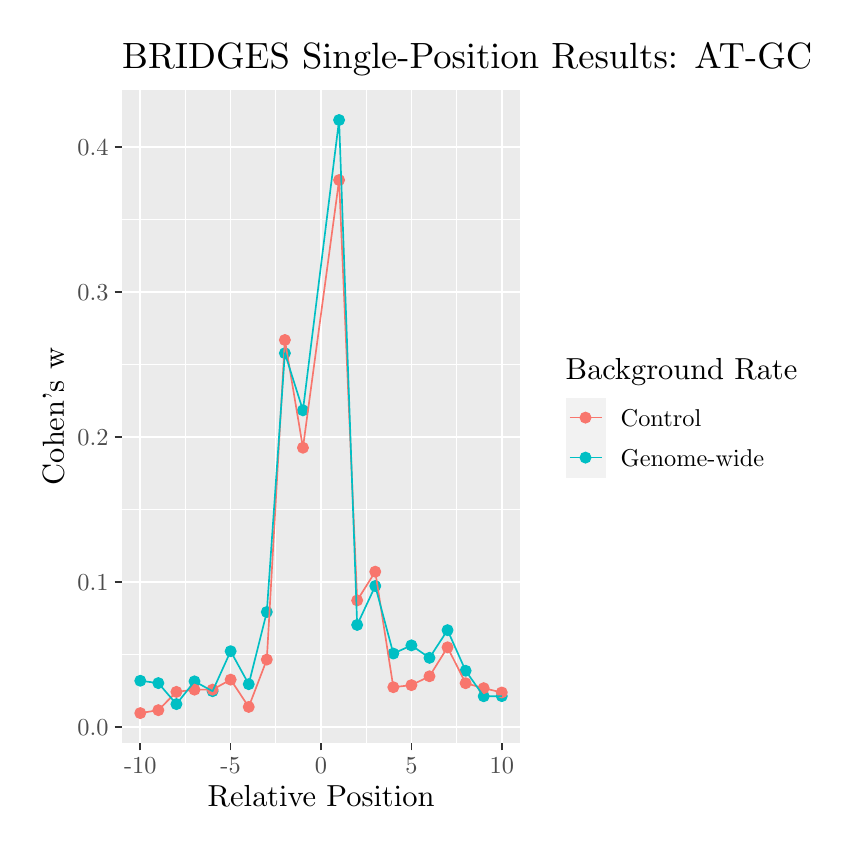
\begin{tikzpicture}[x=1pt,y=1pt]
\definecolor{fillColor}{RGB}{255,255,255}
\path[use as bounding box,fill=fillColor,fill opacity=0.00] (0,0) rectangle (289.08,289.08);
\begin{scope}
\path[clip] (  0.00,  0.00) rectangle (289.08,289.08);
\definecolor{drawColor}{RGB}{255,255,255}
\definecolor{fillColor}{RGB}{255,255,255}

\path[draw=drawColor,line width= 0.6pt,line join=round,line cap=round,fill=fillColor] (  0.00,  0.00) rectangle (289.08,289.08);
\end{scope}
\begin{scope}
\path[clip] ( 34.16, 30.69) rectangle (177.85,266.42);
\definecolor{fillColor}{gray}{0.92}

\path[fill=fillColor] ( 34.16, 30.69) rectangle (177.85,266.42);
\definecolor{drawColor}{RGB}{255,255,255}

\path[draw=drawColor,line width= 0.3pt,line join=round] ( 34.16, 62.67) --
	(177.85, 62.67);

\path[draw=drawColor,line width= 0.3pt,line join=round] ( 34.16,115.02) --
	(177.85,115.02);

\path[draw=drawColor,line width= 0.3pt,line join=round] ( 34.16,167.37) --
	(177.85,167.37);

\path[draw=drawColor,line width= 0.3pt,line join=round] ( 34.16,219.73) --
	(177.85,219.73);

\path[draw=drawColor,line width= 0.3pt,line join=round] ( 57.02, 30.69) --
	( 57.02,266.42);

\path[draw=drawColor,line width= 0.3pt,line join=round] ( 89.67, 30.69) --
	( 89.67,266.42);

\path[draw=drawColor,line width= 0.3pt,line join=round] (122.33, 30.69) --
	(122.33,266.42);

\path[draw=drawColor,line width= 0.3pt,line join=round] (154.99, 30.69) --
	(154.99,266.42);

\path[draw=drawColor,line width= 0.6pt,line join=round] ( 34.16, 36.49) --
	(177.85, 36.49);

\path[draw=drawColor,line width= 0.6pt,line join=round] ( 34.16, 88.85) --
	(177.85, 88.85);

\path[draw=drawColor,line width= 0.6pt,line join=round] ( 34.16,141.20) --
	(177.85,141.20);

\path[draw=drawColor,line width= 0.6pt,line join=round] ( 34.16,193.55) --
	(177.85,193.55);

\path[draw=drawColor,line width= 0.6pt,line join=round] ( 34.16,245.90) --
	(177.85,245.90);

\path[draw=drawColor,line width= 0.6pt,line join=round] ( 40.69, 30.69) --
	( 40.69,266.42);

\path[draw=drawColor,line width= 0.6pt,line join=round] ( 73.34, 30.69) --
	( 73.34,266.42);

\path[draw=drawColor,line width= 0.6pt,line join=round] (106.00, 30.69) --
	(106.00,266.42);

\path[draw=drawColor,line width= 0.6pt,line join=round] (138.66, 30.69) --
	(138.66,266.42);

\path[draw=drawColor,line width= 0.6pt,line join=round] (171.32, 30.69) --
	(171.32,266.42);
\definecolor{drawColor}{RGB}{0,191,196}
\definecolor{fillColor}{RGB}{0,191,196}

\path[draw=drawColor,line width= 0.4pt,line join=round,line cap=round,fill=fillColor] ( 40.69, 53.09) circle (  1.96);
\definecolor{drawColor}{RGB}{248,118,109}
\definecolor{fillColor}{RGB}{248,118,109}

\path[draw=drawColor,line width= 0.4pt,line join=round,line cap=round,fill=fillColor] ( 40.69, 41.40) circle (  1.96);
\definecolor{drawColor}{RGB}{0,191,196}
\definecolor{fillColor}{RGB}{0,191,196}

\path[draw=drawColor,line width= 0.4pt,line join=round,line cap=round,fill=fillColor] ( 47.22, 52.24) circle (  1.96);
\definecolor{drawColor}{RGB}{248,118,109}
\definecolor{fillColor}{RGB}{248,118,109}

\path[draw=drawColor,line width= 0.4pt,line join=round,line cap=round,fill=fillColor] ( 47.22, 42.46) circle (  1.96);
\definecolor{drawColor}{RGB}{0,191,196}
\definecolor{fillColor}{RGB}{0,191,196}

\path[draw=drawColor,line width= 0.4pt,line join=round,line cap=round,fill=fillColor] ( 53.75, 44.65) circle (  1.96);
\definecolor{drawColor}{RGB}{248,118,109}
\definecolor{fillColor}{RGB}{248,118,109}

\path[draw=drawColor,line width= 0.4pt,line join=round,line cap=round,fill=fillColor] ( 53.75, 49.07) circle (  1.96);
\definecolor{drawColor}{RGB}{0,191,196}
\definecolor{fillColor}{RGB}{0,191,196}

\path[draw=drawColor,line width= 0.4pt,line join=round,line cap=round,fill=fillColor] ( 60.28, 52.87) circle (  1.96);
\definecolor{drawColor}{RGB}{248,118,109}
\definecolor{fillColor}{RGB}{248,118,109}

\path[draw=drawColor,line width= 0.4pt,line join=round,line cap=round,fill=fillColor] ( 60.28, 49.87) circle (  1.96);
\definecolor{drawColor}{RGB}{0,191,196}
\definecolor{fillColor}{RGB}{0,191,196}

\path[draw=drawColor,line width= 0.4pt,line join=round,line cap=round,fill=fillColor] ( 66.81, 49.32) circle (  1.96);
\definecolor{drawColor}{RGB}{248,118,109}
\definecolor{fillColor}{RGB}{248,118,109}

\path[draw=drawColor,line width= 0.4pt,line join=round,line cap=round,fill=fillColor] ( 66.81, 49.88) circle (  1.96);
\definecolor{drawColor}{RGB}{0,191,196}
\definecolor{fillColor}{RGB}{0,191,196}

\path[draw=drawColor,line width= 0.4pt,line join=round,line cap=round,fill=fillColor] ( 73.34, 63.77) circle (  1.96);
\definecolor{drawColor}{RGB}{248,118,109}
\definecolor{fillColor}{RGB}{248,118,109}

\path[draw=drawColor,line width= 0.4pt,line join=round,line cap=round,fill=fillColor] ( 73.34, 53.50) circle (  1.96);
\definecolor{drawColor}{RGB}{0,191,196}
\definecolor{fillColor}{RGB}{0,191,196}

\path[draw=drawColor,line width= 0.4pt,line join=round,line cap=round,fill=fillColor] ( 79.88, 51.85) circle (  1.96);
\definecolor{drawColor}{RGB}{248,118,109}
\definecolor{fillColor}{RGB}{248,118,109}

\path[draw=drawColor,line width= 0.4pt,line join=round,line cap=round,fill=fillColor] ( 79.88, 43.63) circle (  1.96);
\definecolor{drawColor}{RGB}{0,191,196}
\definecolor{fillColor}{RGB}{0,191,196}

\path[draw=drawColor,line width= 0.4pt,line join=round,line cap=round,fill=fillColor] ( 86.41, 77.93) circle (  1.96);
\definecolor{drawColor}{RGB}{248,118,109}
\definecolor{fillColor}{RGB}{248,118,109}

\path[draw=drawColor,line width= 0.4pt,line join=round,line cap=round,fill=fillColor] ( 86.41, 60.74) circle (  1.96);
\definecolor{drawColor}{RGB}{0,191,196}
\definecolor{fillColor}{RGB}{0,191,196}

\path[draw=drawColor,line width= 0.4pt,line join=round,line cap=round,fill=fillColor] ( 92.94,171.45) circle (  1.96);
\definecolor{drawColor}{RGB}{248,118,109}
\definecolor{fillColor}{RGB}{248,118,109}

\path[draw=drawColor,line width= 0.4pt,line join=round,line cap=round,fill=fillColor] ( 92.94,176.22) circle (  1.96);
\definecolor{drawColor}{RGB}{0,191,196}
\definecolor{fillColor}{RGB}{0,191,196}

\path[draw=drawColor,line width= 0.4pt,line join=round,line cap=round,fill=fillColor] ( 99.47,150.81) circle (  1.96);
\definecolor{drawColor}{RGB}{248,118,109}
\definecolor{fillColor}{RGB}{248,118,109}

\path[draw=drawColor,line width= 0.4pt,line join=round,line cap=round,fill=fillColor] ( 99.47,137.29) circle (  1.96);
\definecolor{drawColor}{RGB}{0,191,196}
\definecolor{fillColor}{RGB}{0,191,196}

\path[draw=drawColor,line width= 0.4pt,line join=round,line cap=round,fill=fillColor] (112.53,255.71) circle (  1.96);
\definecolor{drawColor}{RGB}{248,118,109}
\definecolor{fillColor}{RGB}{248,118,109}

\path[draw=drawColor,line width= 0.4pt,line join=round,line cap=round,fill=fillColor] (112.53,234.02) circle (  1.96);
\definecolor{drawColor}{RGB}{0,191,196}
\definecolor{fillColor}{RGB}{0,191,196}

\path[draw=drawColor,line width= 0.4pt,line join=round,line cap=round,fill=fillColor] (119.06, 73.26) circle (  1.96);
\definecolor{drawColor}{RGB}{248,118,109}
\definecolor{fillColor}{RGB}{248,118,109}

\path[draw=drawColor,line width= 0.4pt,line join=round,line cap=round,fill=fillColor] (119.06, 82.12) circle (  1.96);
\definecolor{drawColor}{RGB}{0,191,196}
\definecolor{fillColor}{RGB}{0,191,196}

\path[draw=drawColor,line width= 0.4pt,line join=round,line cap=round,fill=fillColor] (125.60, 87.33) circle (  1.96);
\definecolor{drawColor}{RGB}{248,118,109}
\definecolor{fillColor}{RGB}{248,118,109}

\path[draw=drawColor,line width= 0.4pt,line join=round,line cap=round,fill=fillColor] (125.60, 92.50) circle (  1.96);
\definecolor{drawColor}{RGB}{0,191,196}
\definecolor{fillColor}{RGB}{0,191,196}

\path[draw=drawColor,line width= 0.4pt,line join=round,line cap=round,fill=fillColor] (132.13, 62.92) circle (  1.96);
\definecolor{drawColor}{RGB}{248,118,109}
\definecolor{fillColor}{RGB}{248,118,109}

\path[draw=drawColor,line width= 0.4pt,line join=round,line cap=round,fill=fillColor] (132.13, 50.76) circle (  1.96);
\definecolor{drawColor}{RGB}{0,191,196}
\definecolor{fillColor}{RGB}{0,191,196}

\path[draw=drawColor,line width= 0.4pt,line join=round,line cap=round,fill=fillColor] (138.66, 65.87) circle (  1.96);
\definecolor{drawColor}{RGB}{248,118,109}
\definecolor{fillColor}{RGB}{248,118,109}

\path[draw=drawColor,line width= 0.4pt,line join=round,line cap=round,fill=fillColor] (138.66, 51.50) circle (  1.96);
\definecolor{drawColor}{RGB}{0,191,196}
\definecolor{fillColor}{RGB}{0,191,196}

\path[draw=drawColor,line width= 0.4pt,line join=round,line cap=round,fill=fillColor] (145.19, 61.37) circle (  1.96);
\definecolor{drawColor}{RGB}{248,118,109}
\definecolor{fillColor}{RGB}{248,118,109}

\path[draw=drawColor,line width= 0.4pt,line join=round,line cap=round,fill=fillColor] (145.19, 54.70) circle (  1.96);
\definecolor{drawColor}{RGB}{0,191,196}
\definecolor{fillColor}{RGB}{0,191,196}

\path[draw=drawColor,line width= 0.4pt,line join=round,line cap=round,fill=fillColor] (151.72, 71.37) circle (  1.96);
\definecolor{drawColor}{RGB}{248,118,109}
\definecolor{fillColor}{RGB}{248,118,109}

\path[draw=drawColor,line width= 0.4pt,line join=round,line cap=round,fill=fillColor] (151.72, 65.17) circle (  1.96);
\definecolor{drawColor}{RGB}{0,191,196}
\definecolor{fillColor}{RGB}{0,191,196}

\path[draw=drawColor,line width= 0.4pt,line join=round,line cap=round,fill=fillColor] (158.25, 56.70) circle (  1.96);
\definecolor{drawColor}{RGB}{248,118,109}
\definecolor{fillColor}{RGB}{248,118,109}

\path[draw=drawColor,line width= 0.4pt,line join=round,line cap=round,fill=fillColor] (158.25, 52.20) circle (  1.96);
\definecolor{drawColor}{RGB}{0,191,196}
\definecolor{fillColor}{RGB}{0,191,196}

\path[draw=drawColor,line width= 0.4pt,line join=round,line cap=round,fill=fillColor] (164.78, 47.49) circle (  1.96);
\definecolor{drawColor}{RGB}{248,118,109}
\definecolor{fillColor}{RGB}{248,118,109}

\path[draw=drawColor,line width= 0.4pt,line join=round,line cap=round,fill=fillColor] (164.78, 50.41) circle (  1.96);
\definecolor{drawColor}{RGB}{0,191,196}
\definecolor{fillColor}{RGB}{0,191,196}

\path[draw=drawColor,line width= 0.4pt,line join=round,line cap=round,fill=fillColor] (171.32, 47.53) circle (  1.96);
\definecolor{drawColor}{RGB}{248,118,109}
\definecolor{fillColor}{RGB}{248,118,109}

\path[draw=drawColor,line width= 0.4pt,line join=round,line cap=round,fill=fillColor] (171.32, 48.85) circle (  1.96);

\path[draw=drawColor,line width= 0.6pt,line join=round] ( 40.69, 41.40) --
	( 47.22, 42.46) --
	( 53.75, 49.07) --
	( 60.28, 49.87) --
	( 66.81, 49.88) --
	( 73.34, 53.50) --
	( 79.88, 43.63) --
	( 86.41, 60.74) --
	( 92.94,176.22) --
	( 99.47,137.29) --
	(112.53,234.02) --
	(119.06, 82.12) --
	(125.60, 92.50) --
	(132.13, 50.76) --
	(138.66, 51.50) --
	(145.19, 54.70) --
	(151.72, 65.17) --
	(158.25, 52.20) --
	(164.78, 50.41) --
	(171.32, 48.85);
\definecolor{drawColor}{RGB}{0,191,196}

\path[draw=drawColor,line width= 0.6pt,line join=round] ( 40.69, 53.09) --
	( 47.22, 52.24) --
	( 53.75, 44.65) --
	( 60.28, 52.87) --
	( 66.81, 49.32) --
	( 73.34, 63.77) --
	( 79.88, 51.85) --
	( 86.41, 77.93) --
	( 92.94,171.45) --
	( 99.47,150.81) --
	(112.53,255.71) --
	(119.06, 73.26) --
	(125.60, 87.33) --
	(132.13, 62.92) --
	(138.66, 65.87) --
	(145.19, 61.37) --
	(151.72, 71.37) --
	(158.25, 56.70) --
	(164.78, 47.49) --
	(171.32, 47.53);
\end{scope}
\begin{scope}
\path[clip] (  0.00,  0.00) rectangle (289.08,289.08);
\definecolor{drawColor}{gray}{0.30}

\node[text=drawColor,anchor=base east,inner sep=0pt, outer sep=0pt, scale=  0.88] at ( 29.21, 33.46) {0.0};

\node[text=drawColor,anchor=base east,inner sep=0pt, outer sep=0pt, scale=  0.88] at ( 29.21, 85.82) {0.1};

\node[text=drawColor,anchor=base east,inner sep=0pt, outer sep=0pt, scale=  0.88] at ( 29.21,138.17) {0.2};

\node[text=drawColor,anchor=base east,inner sep=0pt, outer sep=0pt, scale=  0.88] at ( 29.21,190.52) {0.3};

\node[text=drawColor,anchor=base east,inner sep=0pt, outer sep=0pt, scale=  0.88] at ( 29.21,242.87) {0.4};
\end{scope}
\begin{scope}
\path[clip] (  0.00,  0.00) rectangle (289.08,289.08);
\definecolor{drawColor}{gray}{0.20}

\path[draw=drawColor,line width= 0.6pt,line join=round] ( 31.41, 36.49) --
	( 34.16, 36.49);

\path[draw=drawColor,line width= 0.6pt,line join=round] ( 31.41, 88.85) --
	( 34.16, 88.85);

\path[draw=drawColor,line width= 0.6pt,line join=round] ( 31.41,141.20) --
	( 34.16,141.20);

\path[draw=drawColor,line width= 0.6pt,line join=round] ( 31.41,193.55) --
	( 34.16,193.55);

\path[draw=drawColor,line width= 0.6pt,line join=round] ( 31.41,245.90) --
	( 34.16,245.90);
\end{scope}
\begin{scope}
\path[clip] (  0.00,  0.00) rectangle (289.08,289.08);
\definecolor{drawColor}{gray}{0.20}

\path[draw=drawColor,line width= 0.6pt,line join=round] ( 40.69, 27.94) --
	( 40.69, 30.69);

\path[draw=drawColor,line width= 0.6pt,line join=round] ( 73.34, 27.94) --
	( 73.34, 30.69);

\path[draw=drawColor,line width= 0.6pt,line join=round] (106.00, 27.94) --
	(106.00, 30.69);

\path[draw=drawColor,line width= 0.6pt,line join=round] (138.66, 27.94) --
	(138.66, 30.69);

\path[draw=drawColor,line width= 0.6pt,line join=round] (171.32, 27.94) --
	(171.32, 30.69);
\end{scope}
\begin{scope}
\path[clip] (  0.00,  0.00) rectangle (289.08,289.08);
\definecolor{drawColor}{gray}{0.30}

\node[text=drawColor,anchor=base,inner sep=0pt, outer sep=0pt, scale=  0.88] at ( 40.69, 19.68) {-10};

\node[text=drawColor,anchor=base,inner sep=0pt, outer sep=0pt, scale=  0.88] at ( 73.34, 19.68) {-5};

\node[text=drawColor,anchor=base,inner sep=0pt, outer sep=0pt, scale=  0.88] at (106.00, 19.68) {0};

\node[text=drawColor,anchor=base,inner sep=0pt, outer sep=0pt, scale=  0.88] at (138.66, 19.68) {5};

\node[text=drawColor,anchor=base,inner sep=0pt, outer sep=0pt, scale=  0.88] at (171.32, 19.68) {10};
\end{scope}
\begin{scope}
\path[clip] (  0.00,  0.00) rectangle (289.08,289.08);
\definecolor{drawColor}{RGB}{0,0,0}

\node[text=drawColor,anchor=base,inner sep=0pt, outer sep=0pt, scale=  1.10] at (106.00,  7.64) {Relative Position};
\end{scope}
\begin{scope}
\path[clip] (  0.00,  0.00) rectangle (289.08,289.08);
\definecolor{drawColor}{RGB}{0,0,0}

\node[text=drawColor,rotate= 90.00,anchor=base,inner sep=0pt, outer sep=0pt, scale=  1.10] at ( 13.08,148.55) {Cohen's w};
\end{scope}
\begin{scope}
\path[clip] (  0.00,  0.00) rectangle (289.08,289.08);
\definecolor{fillColor}{RGB}{255,255,255}

\path[fill=fillColor] (188.85,120.99) rectangle (283.58,176.12);
\end{scope}
\begin{scope}
\path[clip] (  0.00,  0.00) rectangle (289.08,289.08);
\definecolor{drawColor}{RGB}{0,0,0}

\node[text=drawColor,anchor=base west,inner sep=0pt, outer sep=0pt, scale=  1.10] at (194.35,161.97) {Background Rate};
\end{scope}
\begin{scope}
\path[clip] (  0.00,  0.00) rectangle (289.08,289.08);
\definecolor{fillColor}{gray}{0.95}

\path[fill=fillColor] (194.35,140.95) rectangle (208.80,155.40);
\end{scope}
\begin{scope}
\path[clip] (  0.00,  0.00) rectangle (289.08,289.08);
\definecolor{drawColor}{RGB}{248,118,109}
\definecolor{fillColor}{RGB}{248,118,109}

\path[draw=drawColor,line width= 0.4pt,line join=round,line cap=round,fill=fillColor] (201.57,148.17) circle (  1.96);
\end{scope}
\begin{scope}
\path[clip] (  0.00,  0.00) rectangle (289.08,289.08);
\definecolor{drawColor}{RGB}{248,118,109}

\path[draw=drawColor,line width= 0.6pt,line join=round] (195.79,148.17) -- (207.36,148.17);
\end{scope}
\begin{scope}
\path[clip] (  0.00,  0.00) rectangle (289.08,289.08);
\definecolor{fillColor}{gray}{0.95}

\path[fill=fillColor] (194.35,126.49) rectangle (208.80,140.95);
\end{scope}
\begin{scope}
\path[clip] (  0.00,  0.00) rectangle (289.08,289.08);
\definecolor{drawColor}{RGB}{0,191,196}
\definecolor{fillColor}{RGB}{0,191,196}

\path[draw=drawColor,line width= 0.4pt,line join=round,line cap=round,fill=fillColor] (201.57,133.72) circle (  1.96);
\end{scope}
\begin{scope}
\path[clip] (  0.00,  0.00) rectangle (289.08,289.08);
\definecolor{drawColor}{RGB}{0,191,196}

\path[draw=drawColor,line width= 0.6pt,line join=round] (195.79,133.72) -- (207.36,133.72);
\end{scope}
\begin{scope}
\path[clip] (  0.00,  0.00) rectangle (289.08,289.08);
\definecolor{drawColor}{RGB}{0,0,0}

\node[text=drawColor,anchor=base west,inner sep=0pt, outer sep=0pt, scale=  0.88] at (214.30,145.14) {Control};
\end{scope}
\begin{scope}
\path[clip] (  0.00,  0.00) rectangle (289.08,289.08);
\definecolor{drawColor}{RGB}{0,0,0}

\node[text=drawColor,anchor=base west,inner sep=0pt, outer sep=0pt, scale=  0.88] at (214.30,130.69) {Genome-wide};
\end{scope}
\begin{scope}
\path[clip] (  0.00,  0.00) rectangle (289.08,289.08);
\definecolor{drawColor}{RGB}{0,0,0}

\node[text=drawColor,anchor=base west,inner sep=0pt, outer sep=0pt, scale=  1.32] at ( 34.16,274.49) {BRIDGES Single-Position Results: AT-GC};
\end{scope}
\end{tikzpicture}
